\documentclass[12pt]{article}
\usepackage{latexblog}

% ============================================================
% Blog Metadata
% ============================================================
\blogtitle{TCP(2)：TCP报文实例}
\blogdate{2020-09-14}
\blogtags{TCP/IP, 刨根问底, 协议}
\bloglang{zh}
\blogsummary{}

\begin{document}
\makeblogtitle

TCP每个报文都有一个序列号，这个序列号在初始的时候是随机生成的（而不是直接使用0或者1），那么这样做的原因究竟是为什么？

\section{TCP 实例}\label{tcp-ux5b9eux4f8b}

使用\href{https://www.wireshark.org/}{Wireshark}和\href{https://sourceforge.net/projects/sockettest/}{SocketTest}在本地进行数据发送和接收，可以抓取到TCP报文。首先使用SocketTest在本地(127.0.0.1)的10240端口上启动一个Socket服务器，然后使用它的客户端功能连接这个端口，并在Wireshark中监听本地回环网卡(localhost)，即可抓取到对应的数据包。

\subsection{三次握手}\label{ux4e09ux6b21ux63e1ux624b}

\begin{figure}
\centering
\pandocbounded{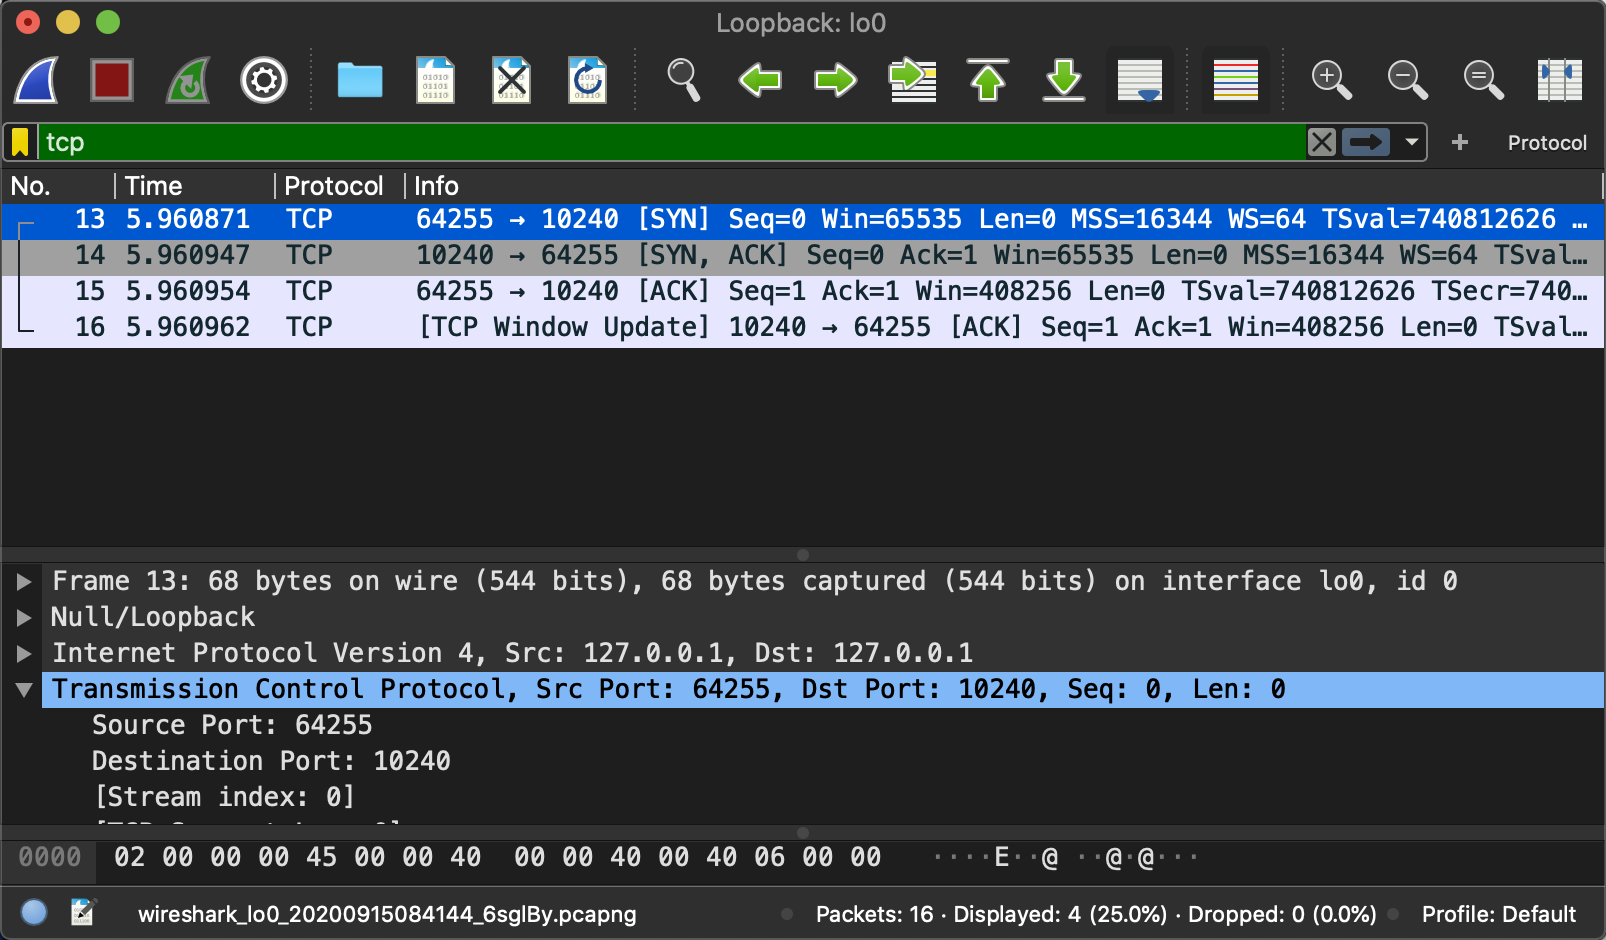
\includegraphics[keepaspectratio,alt={3-way Handshake}]{images/Wireshark-lo-1.png}}
\caption{3-way Handshake}
\end{figure}

可以看出，是一个标准的三次握手的过程，握手完成之后，服务端给客户端发送了一个Window Update。

\subsubsection{1:客户端发送SYN}\label{ux5ba2ux6237ux7aefux53d1ux9001syn}

\begin{Shaded}
\begin{Highlighting}[]
\VariableTok{Frame} \DecValTok{13}\OperatorTok{:} \DecValTok{68} \VariableTok{bytes} \VariableTok{on}\NormalTok{ wire }\OperatorTok{(}\DecValTok{544} \VariableTok{bits}\OperatorTok{),} \DecValTok{68} \VariableTok{bytes}\NormalTok{ captured }\OperatorTok{(}\DecValTok{544} \VariableTok{bits}\OperatorTok{)} \VariableTok{on} \VariableTok{interface} \VariableTok{lo0}\OperatorTok{,} \VariableTok{id} \DecValTok{0}
\VariableTok{Null}\OperatorTok{/}\VariableTok{Loopback}
\VariableTok{Internet} \VariableTok{Protocol} \VariableTok{Version} \DecValTok{4}\OperatorTok{,} \VariableTok{Src}\OperatorTok{:} \DecValTok{127.0.0.1}\OperatorTok{,} \VariableTok{Dst}\OperatorTok{:} \DecValTok{127.0.0.1}
\VariableTok{Transmission} \VariableTok{Control} \VariableTok{Protocol}\OperatorTok{,} \VariableTok{Src} \VariableTok{Port}\OperatorTok{:} \DecValTok{64255}\OperatorTok{,} \VariableTok{Dst} \VariableTok{Port}\OperatorTok{:} \DecValTok{10240}\OperatorTok{,} \VariableTok{Seq}\OperatorTok{:} \DecValTok{0}\OperatorTok{,} \VariableTok{Len}\OperatorTok{:} \DecValTok{0}
    \VariableTok{Source} \VariableTok{Port}\OperatorTok{:} \DecValTok{64255}
    \VariableTok{Destination} \VariableTok{Port}\OperatorTok{:} \DecValTok{10240}
    \OperatorTok{[}\VariableTok{Stream} \VariableTok{index}\OperatorTok{:} \DecValTok{0}\OperatorTok{]}
    \OperatorTok{[}\ConstantTok{TCP} \VariableTok{Segment} \VariableTok{Len}\OperatorTok{:} \DecValTok{0}\OperatorTok{]}
    \VariableTok{Sequence} \VariableTok{number}\OperatorTok{:} \DecValTok{0}    \OperatorTok{(}\VariableTok{relative} \VariableTok{sequence} \VariableTok{number}\OperatorTok{)}
    \VariableTok{Sequence}\NormalTok{ number }\OperatorTok{(}\VariableTok{raw}\OperatorTok{):} \DecValTok{3261314628}
    \OperatorTok{[}\VariableTok{Next} \VariableTok{sequence} \VariableTok{number}\OperatorTok{:} \DecValTok{1}    \OperatorTok{(}\VariableTok{relative} \VariableTok{sequence} \VariableTok{number}\OperatorTok{)]}
    \VariableTok{Acknowledgment} \VariableTok{number}\OperatorTok{:} \DecValTok{0}
    \VariableTok{Acknowledgment}\NormalTok{ number }\OperatorTok{(}\VariableTok{raw}\OperatorTok{):} \DecValTok{0}
    \DecValTok{1011} \OperatorTok{....} \OperatorTok{=} \VariableTok{Header} \VariableTok{Length}\OperatorTok{:} \DecValTok{44}\NormalTok{ bytes }\OperatorTok{(}\DecValTok{11}\OperatorTok{)}
    \VariableTok{Flags}\OperatorTok{:} \DecValTok{0x002} \OperatorTok{(}\ConstantTok{SYN}\OperatorTok{)}
    \VariableTok{Window} \VariableTok{size} \VariableTok{value}\OperatorTok{:} \DecValTok{65535}
    \OperatorTok{[}\VariableTok{Calculated} \VariableTok{window} \VariableTok{size}\OperatorTok{:} \DecValTok{65535}\OperatorTok{]}
    \VariableTok{Checksum}\OperatorTok{:} \DecValTok{0xfe34} \OperatorTok{[}\VariableTok{unverified}\OperatorTok{]}
    \OperatorTok{[}\VariableTok{Checksum} \VariableTok{Status}\OperatorTok{:} \VariableTok{Unverified}\OperatorTok{]}
    \VariableTok{Urgent} \VariableTok{pointer}\OperatorTok{:} \DecValTok{0}
    \VariableTok{Options}\OperatorTok{:} \OperatorTok{(}\DecValTok{24} \VariableTok{bytes}\OperatorTok{),} \VariableTok{Maximum} \VariableTok{segment} \VariableTok{size}\OperatorTok{,} \VariableTok{No}\OperatorTok{{-}}\NormalTok{Operation }\OperatorTok{(}\ConstantTok{NOP}\OperatorTok{),} \VariableTok{Window} \VariableTok{scale}\OperatorTok{,} \VariableTok{No}\OperatorTok{{-}}\NormalTok{Operation }\OperatorTok{(}\ConstantTok{NOP}\OperatorTok{),} \VariableTok{No}\OperatorTok{{-}}\NormalTok{Operation }\OperatorTok{(}\ConstantTok{NOP}\OperatorTok{),} \VariableTok{Timestamps}\OperatorTok{,} \ConstantTok{SACK} \VariableTok{permitted}\OperatorTok{,} \VariableTok{End} \VariableTok{of} \VariableTok{Option}\NormalTok{ List }\OperatorTok{(}\ConstantTok{EOL}\OperatorTok{)}
        \ConstantTok{TCP} \VariableTok{Option} \OperatorTok{{-}} \VariableTok{Maximum} \VariableTok{segment} \VariableTok{size}\OperatorTok{:} \DecValTok{16344} \VariableTok{bytes}
        \ConstantTok{TCP} \VariableTok{Option} \OperatorTok{{-}} \VariableTok{No}\OperatorTok{{-}}\NormalTok{Operation }\OperatorTok{(}\ConstantTok{NOP}\OperatorTok{)}
        \ConstantTok{TCP} \VariableTok{Option} \OperatorTok{{-}} \VariableTok{Window} \VariableTok{scale}\OperatorTok{:} \DecValTok{6} \OperatorTok{(}\VariableTok{multiply} \VariableTok{by} \DecValTok{64}\OperatorTok{)}
        \ConstantTok{TCP} \VariableTok{Option} \OperatorTok{{-}} \VariableTok{No}\OperatorTok{{-}}\NormalTok{Operation }\OperatorTok{(}\ConstantTok{NOP}\OperatorTok{)}
        \ConstantTok{TCP} \VariableTok{Option} \OperatorTok{{-}} \VariableTok{No}\OperatorTok{{-}}\NormalTok{Operation }\OperatorTok{(}\ConstantTok{NOP}\OperatorTok{)}
        \ConstantTok{TCP} \VariableTok{Option} \OperatorTok{{-}} \VariableTok{Timestamps}\OperatorTok{:} \VariableTok{TSval} \DecValTok{740812626}\OperatorTok{,} \VariableTok{TSecr} \DecValTok{0}
        \ConstantTok{TCP} \VariableTok{Option} \OperatorTok{{-}} \ConstantTok{SACK} \VariableTok{permitted}
        \ConstantTok{TCP} \VariableTok{Option} \OperatorTok{{-}} \VariableTok{End} \VariableTok{of} \VariableTok{Option}\NormalTok{ List }\OperatorTok{(}\ConstantTok{EOL}\OperatorTok{)}
    \OperatorTok{[}\VariableTok{Timestamps}\OperatorTok{]}
\end{Highlighting}
\end{Shaded}

\subsubsection{2:服务端回复SYN/ACK}\label{ux670dux52a1ux7aefux56deux590dsynack}

\begin{Shaded}
\begin{Highlighting}[]
\VariableTok{Frame} \DecValTok{14}\OperatorTok{:} \DecValTok{68} \VariableTok{bytes} \VariableTok{on}\NormalTok{ wire }\OperatorTok{(}\DecValTok{544} \VariableTok{bits}\OperatorTok{),} \DecValTok{68} \VariableTok{bytes}\NormalTok{ captured }\OperatorTok{(}\DecValTok{544} \VariableTok{bits}\OperatorTok{)} \VariableTok{on} \VariableTok{interface} \VariableTok{lo0}\OperatorTok{,} \VariableTok{id} \DecValTok{0}
\VariableTok{Null}\OperatorTok{/}\VariableTok{Loopback}
\VariableTok{Internet} \VariableTok{Protocol} \VariableTok{Version} \DecValTok{4}\OperatorTok{,} \VariableTok{Src}\OperatorTok{:} \DecValTok{127.0.0.1}\OperatorTok{,} \VariableTok{Dst}\OperatorTok{:} \DecValTok{127.0.0.1}
\VariableTok{Transmission} \VariableTok{Control} \VariableTok{Protocol}\OperatorTok{,} \VariableTok{Src} \VariableTok{Port}\OperatorTok{:} \DecValTok{10240}\OperatorTok{,} \VariableTok{Dst} \VariableTok{Port}\OperatorTok{:} \DecValTok{64255}\OperatorTok{,} \VariableTok{Seq}\OperatorTok{:} \DecValTok{0}\OperatorTok{,} \VariableTok{Ack}\OperatorTok{:} \DecValTok{1}\OperatorTok{,} \VariableTok{Len}\OperatorTok{:} \DecValTok{0}
    \VariableTok{Source} \VariableTok{Port}\OperatorTok{:} \DecValTok{10240}
    \VariableTok{Destination} \VariableTok{Port}\OperatorTok{:} \DecValTok{64255}
    \OperatorTok{[}\VariableTok{Stream} \VariableTok{index}\OperatorTok{:} \DecValTok{0}\OperatorTok{]}
    \OperatorTok{[}\ConstantTok{TCP} \VariableTok{Segment} \VariableTok{Len}\OperatorTok{:} \DecValTok{0}\OperatorTok{]}
    \VariableTok{Sequence} \VariableTok{number}\OperatorTok{:} \DecValTok{0}    \OperatorTok{(}\VariableTok{relative} \VariableTok{sequence} \VariableTok{number}\OperatorTok{)}
    \VariableTok{Sequence}\NormalTok{ number }\OperatorTok{(}\VariableTok{raw}\OperatorTok{):} \DecValTok{1175996045}
    \OperatorTok{[}\VariableTok{Next} \VariableTok{sequence} \VariableTok{number}\OperatorTok{:} \DecValTok{1}    \OperatorTok{(}\VariableTok{relative} \VariableTok{sequence} \VariableTok{number}\OperatorTok{)]}
    \VariableTok{Acknowledgment} \VariableTok{number}\OperatorTok{:} \DecValTok{1}    \OperatorTok{(}\VariableTok{relative} \VariableTok{ack} \VariableTok{number}\OperatorTok{)}
    \VariableTok{Acknowledgment}\NormalTok{ number }\OperatorTok{(}\VariableTok{raw}\OperatorTok{):} \DecValTok{3261314629}
    \DecValTok{1011} \OperatorTok{....} \OperatorTok{=} \VariableTok{Header} \VariableTok{Length}\OperatorTok{:} \DecValTok{44}\NormalTok{ bytes }\OperatorTok{(}\DecValTok{11}\OperatorTok{)}
    \VariableTok{Flags}\OperatorTok{:} \DecValTok{0x012} \OperatorTok{(}\ConstantTok{SYN}\OperatorTok{,} \ConstantTok{ACK}\OperatorTok{)}
    \VariableTok{Window} \VariableTok{size} \VariableTok{value}\OperatorTok{:} \DecValTok{65535}
    \OperatorTok{[}\VariableTok{Calculated} \VariableTok{window} \VariableTok{size}\OperatorTok{:} \DecValTok{65535}\OperatorTok{]}
    \VariableTok{Checksum}\OperatorTok{:} \DecValTok{0xfe34} \OperatorTok{[}\VariableTok{unverified}\OperatorTok{]}
    \OperatorTok{[}\VariableTok{Checksum} \VariableTok{Status}\OperatorTok{:} \VariableTok{Unverified}\OperatorTok{]}
    \VariableTok{Urgent} \VariableTok{pointer}\OperatorTok{:} \DecValTok{0}
    \VariableTok{Options}\OperatorTok{:} \OperatorTok{(}\DecValTok{24} \VariableTok{bytes}\OperatorTok{),} \VariableTok{Maximum} \VariableTok{segment} \VariableTok{size}\OperatorTok{,} \VariableTok{No}\OperatorTok{{-}}\NormalTok{Operation }\OperatorTok{(}\ConstantTok{NOP}\OperatorTok{),} \VariableTok{Window} \VariableTok{scale}\OperatorTok{,} \VariableTok{No}\OperatorTok{{-}}\NormalTok{Operation }\OperatorTok{(}\ConstantTok{NOP}\OperatorTok{),} \VariableTok{No}\OperatorTok{{-}}\NormalTok{Operation }\OperatorTok{(}\ConstantTok{NOP}\OperatorTok{),} \VariableTok{Timestamps}\OperatorTok{,} \ConstantTok{SACK} \VariableTok{permitted}\OperatorTok{,} \VariableTok{End} \VariableTok{of} \VariableTok{Option}\NormalTok{ List }\OperatorTok{(}\ConstantTok{EOL}\OperatorTok{)}
        \ConstantTok{TCP} \VariableTok{Option} \OperatorTok{{-}} \VariableTok{Maximum} \VariableTok{segment} \VariableTok{size}\OperatorTok{:} \DecValTok{16344} \VariableTok{bytes}
        \ConstantTok{TCP} \VariableTok{Option} \OperatorTok{{-}} \VariableTok{No}\OperatorTok{{-}}\NormalTok{Operation }\OperatorTok{(}\ConstantTok{NOP}\OperatorTok{)}
        \ConstantTok{TCP} \VariableTok{Option} \OperatorTok{{-}} \VariableTok{Window} \VariableTok{scale}\OperatorTok{:} \DecValTok{6} \OperatorTok{(}\VariableTok{multiply} \VariableTok{by} \DecValTok{64}\OperatorTok{)}
        \ConstantTok{TCP} \VariableTok{Option} \OperatorTok{{-}} \VariableTok{No}\OperatorTok{{-}}\NormalTok{Operation }\OperatorTok{(}\ConstantTok{NOP}\OperatorTok{)}
        \ConstantTok{TCP} \VariableTok{Option} \OperatorTok{{-}} \VariableTok{No}\OperatorTok{{-}}\NormalTok{Operation }\OperatorTok{(}\ConstantTok{NOP}\OperatorTok{)}
        \ConstantTok{TCP} \VariableTok{Option} \OperatorTok{{-}} \VariableTok{Timestamps}\OperatorTok{:} \VariableTok{TSval} \DecValTok{740812626}\OperatorTok{,} \VariableTok{TSecr} \DecValTok{740812626}
        \ConstantTok{TCP} \VariableTok{Option} \OperatorTok{{-}} \ConstantTok{SACK} \VariableTok{permitted}
        \ConstantTok{TCP} \VariableTok{Option} \OperatorTok{{-}} \VariableTok{End} \VariableTok{of} \VariableTok{Option}\NormalTok{ List }\OperatorTok{(}\ConstantTok{EOL}\OperatorTok{)}
    \OperatorTok{[}\ConstantTok{SEQ}\OperatorTok{/}\ConstantTok{ACK} \VariableTok{analysis}\OperatorTok{]}
    \OperatorTok{[}\VariableTok{Timestamps}\OperatorTok{]}
\end{Highlighting}
\end{Shaded}

\subsubsection{3:客户端回复ACK}\label{ux5ba2ux6237ux7aefux56deux590dack}

\begin{Shaded}
\begin{Highlighting}[]
\VariableTok{Frame} \DecValTok{15}\OperatorTok{:} \DecValTok{56} \VariableTok{bytes} \VariableTok{on}\NormalTok{ wire }\OperatorTok{(}\DecValTok{448} \VariableTok{bits}\OperatorTok{),} \DecValTok{56} \VariableTok{bytes}\NormalTok{ captured }\OperatorTok{(}\DecValTok{448} \VariableTok{bits}\OperatorTok{)} \VariableTok{on} \VariableTok{interface} \VariableTok{lo0}\OperatorTok{,} \VariableTok{id} \DecValTok{0}
\VariableTok{Null}\OperatorTok{/}\VariableTok{Loopback}
\VariableTok{Internet} \VariableTok{Protocol} \VariableTok{Version} \DecValTok{4}\OperatorTok{,} \VariableTok{Src}\OperatorTok{:} \DecValTok{127.0.0.1}\OperatorTok{,} \VariableTok{Dst}\OperatorTok{:} \DecValTok{127.0.0.1}
\VariableTok{Transmission} \VariableTok{Control} \VariableTok{Protocol}\OperatorTok{,} \VariableTok{Src} \VariableTok{Port}\OperatorTok{:} \DecValTok{64255}\OperatorTok{,} \VariableTok{Dst} \VariableTok{Port}\OperatorTok{:} \DecValTok{10240}\OperatorTok{,} \VariableTok{Seq}\OperatorTok{:} \DecValTok{1}\OperatorTok{,} \VariableTok{Ack}\OperatorTok{:} \DecValTok{1}\OperatorTok{,} \VariableTok{Len}\OperatorTok{:} \DecValTok{0}
    \VariableTok{Source} \VariableTok{Port}\OperatorTok{:} \DecValTok{64255}
    \VariableTok{Destination} \VariableTok{Port}\OperatorTok{:} \DecValTok{10240}
    \OperatorTok{[}\VariableTok{Stream} \VariableTok{index}\OperatorTok{:} \DecValTok{0}\OperatorTok{]}
    \OperatorTok{[}\ConstantTok{TCP} \VariableTok{Segment} \VariableTok{Len}\OperatorTok{:} \DecValTok{0}\OperatorTok{]}
    \VariableTok{Sequence} \VariableTok{number}\OperatorTok{:} \DecValTok{1}    \OperatorTok{(}\VariableTok{relative} \VariableTok{sequence} \VariableTok{number}\OperatorTok{)}
    \VariableTok{Sequence}\NormalTok{ number }\OperatorTok{(}\VariableTok{raw}\OperatorTok{):} \DecValTok{3261314629}
    \OperatorTok{[}\VariableTok{Next} \VariableTok{sequence} \VariableTok{number}\OperatorTok{:} \DecValTok{1}    \OperatorTok{(}\VariableTok{relative} \VariableTok{sequence} \VariableTok{number}\OperatorTok{)]}
    \VariableTok{Acknowledgment} \VariableTok{number}\OperatorTok{:} \DecValTok{1}    \OperatorTok{(}\VariableTok{relative} \VariableTok{ack} \VariableTok{number}\OperatorTok{)}
    \VariableTok{Acknowledgment}\NormalTok{ number }\OperatorTok{(}\VariableTok{raw}\OperatorTok{):} \DecValTok{1175996046}
    \DecValTok{1000} \OperatorTok{....} \OperatorTok{=} \VariableTok{Header} \VariableTok{Length}\OperatorTok{:} \DecValTok{32}\NormalTok{ bytes }\OperatorTok{(}\DecValTok{8}\OperatorTok{)}
    \VariableTok{Flags}\OperatorTok{:} \DecValTok{0x010} \OperatorTok{(}\ConstantTok{ACK}\OperatorTok{)}
    \VariableTok{Window} \VariableTok{size} \VariableTok{value}\OperatorTok{:} \DecValTok{6379}
    \OperatorTok{[}\VariableTok{Calculated} \VariableTok{window} \VariableTok{size}\OperatorTok{:} \DecValTok{408256}\OperatorTok{]}
    \OperatorTok{[}\VariableTok{Window} \VariableTok{size} \VariableTok{scaling} \VariableTok{factor}\OperatorTok{:} \DecValTok{64}\OperatorTok{]}
    \VariableTok{Checksum}\OperatorTok{:} \DecValTok{0xfe28} \OperatorTok{[}\VariableTok{unverified}\OperatorTok{]}
    \OperatorTok{[}\VariableTok{Checksum} \VariableTok{Status}\OperatorTok{:} \VariableTok{Unverified}\OperatorTok{]}
    \VariableTok{Urgent} \VariableTok{pointer}\OperatorTok{:} \DecValTok{0}
    \VariableTok{Options}\OperatorTok{:} \OperatorTok{(}\DecValTok{12} \VariableTok{bytes}\OperatorTok{),} \VariableTok{No}\OperatorTok{{-}}\NormalTok{Operation }\OperatorTok{(}\ConstantTok{NOP}\OperatorTok{),} \VariableTok{No}\OperatorTok{{-}}\NormalTok{Operation }\OperatorTok{(}\ConstantTok{NOP}\OperatorTok{),} \VariableTok{Timestamps}
        \ConstantTok{TCP} \VariableTok{Option} \OperatorTok{{-}} \VariableTok{No}\OperatorTok{{-}}\NormalTok{Operation }\OperatorTok{(}\ConstantTok{NOP}\OperatorTok{)}
        \ConstantTok{TCP} \VariableTok{Option} \OperatorTok{{-}} \VariableTok{No}\OperatorTok{{-}}\NormalTok{Operation }\OperatorTok{(}\ConstantTok{NOP}\OperatorTok{)}
        \ConstantTok{TCP} \VariableTok{Option} \OperatorTok{{-}} \VariableTok{Timestamps}\OperatorTok{:} \VariableTok{TSval} \DecValTok{740812626}\OperatorTok{,} \VariableTok{TSecr} \DecValTok{740812626}
    \OperatorTok{[}\ConstantTok{SEQ}\OperatorTok{/}\ConstantTok{ACK} \VariableTok{analysis}\OperatorTok{]}
    \OperatorTok{[}\VariableTok{Timestamps}\OperatorTok{]}
\end{Highlighting}
\end{Shaded}

\subsection{数据发送}\label{ux6570ux636eux53d1ux9001}

通过像服务器发送一个''helloworld''来查看数据是如何发送的：

\subsubsection{1:客户端发送PSH/ACK}\label{ux5ba2ux6237ux7aefux53d1ux9001pshack}

\begin{Shaded}
\begin{Highlighting}[]
\VariableTok{Transmission} \VariableTok{Control} \VariableTok{Protocol}\OperatorTok{,} \VariableTok{Src} \VariableTok{Port}\OperatorTok{:} \DecValTok{64255}\OperatorTok{,} \VariableTok{Dst} \VariableTok{Port}\OperatorTok{:} \DecValTok{10240}\OperatorTok{,} \VariableTok{Seq}\OperatorTok{:} \DecValTok{1}\OperatorTok{,} \VariableTok{Ack}\OperatorTok{:} \DecValTok{1}\OperatorTok{,} \VariableTok{Len}\OperatorTok{:} \DecValTok{12}
    \VariableTok{Source} \VariableTok{Port}\OperatorTok{:} \DecValTok{64255}
    \VariableTok{Destination} \VariableTok{Port}\OperatorTok{:} \DecValTok{10240}
    \OperatorTok{[}\VariableTok{Stream} \VariableTok{index}\OperatorTok{:} \DecValTok{0}\OperatorTok{]}
    \OperatorTok{[}\ConstantTok{TCP} \VariableTok{Segment} \VariableTok{Len}\OperatorTok{:} \DecValTok{12}\OperatorTok{]}
    \VariableTok{Sequence} \VariableTok{number}\OperatorTok{:} \DecValTok{1}    \OperatorTok{(}\VariableTok{relative} \VariableTok{sequence} \VariableTok{number}\OperatorTok{)}
    \VariableTok{Sequence}\NormalTok{ number }\OperatorTok{(}\VariableTok{raw}\OperatorTok{):} \DecValTok{3261314629}
    \OperatorTok{[}\VariableTok{Next} \VariableTok{sequence} \VariableTok{number}\OperatorTok{:} \DecValTok{13}    \OperatorTok{(}\VariableTok{relative} \VariableTok{sequence} \VariableTok{number}\OperatorTok{)]}
    \VariableTok{Acknowledgment} \VariableTok{number}\OperatorTok{:} \DecValTok{1}    \OperatorTok{(}\VariableTok{relative} \VariableTok{ack} \VariableTok{number}\OperatorTok{)}
    \VariableTok{Acknowledgment}\NormalTok{ number }\OperatorTok{(}\VariableTok{raw}\OperatorTok{):} \DecValTok{1175996046}
    \DecValTok{1000} \OperatorTok{....} \OperatorTok{=} \VariableTok{Header} \VariableTok{Length}\OperatorTok{:} \DecValTok{32}\NormalTok{ bytes }\OperatorTok{(}\DecValTok{8}\OperatorTok{)}
    \VariableTok{Flags}\OperatorTok{:} \DecValTok{0x018} \OperatorTok{(}\ConstantTok{PSH}\OperatorTok{,} \ConstantTok{ACK}\OperatorTok{)}
    \VariableTok{Window} \VariableTok{size} \VariableTok{value}\OperatorTok{:} \DecValTok{6379}
    \OperatorTok{[}\VariableTok{Calculated} \VariableTok{window} \VariableTok{size}\OperatorTok{:} \DecValTok{6379}\OperatorTok{]}
    \OperatorTok{[}\VariableTok{Window} \VariableTok{size} \VariableTok{scaling} \VariableTok{factor}\OperatorTok{:} \OperatorTok{{-}}\DecValTok{1} \OperatorTok{(}\VariableTok{unknown}\OperatorTok{)]}
    \VariableTok{Checksum}\OperatorTok{:} \DecValTok{0xfe34} \OperatorTok{[}\VariableTok{unverified}\OperatorTok{]}
    \OperatorTok{[}\VariableTok{Checksum} \VariableTok{Status}\OperatorTok{:} \VariableTok{Unverified}\OperatorTok{]}
    \VariableTok{Urgent} \VariableTok{pointer}\OperatorTok{:} \DecValTok{0}
    \VariableTok{Options}\OperatorTok{:} \OperatorTok{(}\DecValTok{12} \VariableTok{bytes}\OperatorTok{),} \VariableTok{No}\OperatorTok{{-}}\NormalTok{Operation }\OperatorTok{(}\ConstantTok{NOP}\OperatorTok{),} \VariableTok{No}\OperatorTok{{-}}\NormalTok{Operation }\OperatorTok{(}\ConstantTok{NOP}\OperatorTok{),} \VariableTok{Timestamps}
        \ConstantTok{TCP} \VariableTok{Option} \OperatorTok{{-}} \VariableTok{No}\OperatorTok{{-}}\NormalTok{Operation }\OperatorTok{(}\ConstantTok{NOP}\OperatorTok{)}
        \ConstantTok{TCP} \VariableTok{Option} \OperatorTok{{-}} \VariableTok{No}\OperatorTok{{-}}\NormalTok{Operation }\OperatorTok{(}\ConstantTok{NOP}\OperatorTok{)}
        \ConstantTok{TCP} \VariableTok{Option} \OperatorTok{{-}} \VariableTok{Timestamps}\OperatorTok{:} \VariableTok{TSval} \DecValTok{742069804}\OperatorTok{,} \VariableTok{TSecr} \DecValTok{740812626}
    \OperatorTok{[}\ConstantTok{SEQ}\OperatorTok{/}\ConstantTok{ACK} \VariableTok{analysis}\OperatorTok{]}
    \OperatorTok{[}\VariableTok{Timestamps}\OperatorTok{]}
    \ConstantTok{TCP}\NormalTok{ payload }\OperatorTok{(}\DecValTok{12} \VariableTok{bytes}\OperatorTok{)}
\end{Highlighting}
\end{Shaded}

\subsubsection{2:服务端回复ACK}\label{ux670dux52a1ux7aefux56deux590dack}

\begin{Shaded}
\begin{Highlighting}[]
\VariableTok{Transmission} \VariableTok{Control} \VariableTok{Protocol}\OperatorTok{,} \VariableTok{Src} \VariableTok{Port}\OperatorTok{:} \DecValTok{10240}\OperatorTok{,} \VariableTok{Dst} \VariableTok{Port}\OperatorTok{:} \DecValTok{64255}\OperatorTok{,} \VariableTok{Seq}\OperatorTok{:} \DecValTok{1}\OperatorTok{,} \VariableTok{Ack}\OperatorTok{:} \DecValTok{13}\OperatorTok{,} \VariableTok{Len}\OperatorTok{:} \DecValTok{0}
    \VariableTok{Source} \VariableTok{Port}\OperatorTok{:} \DecValTok{10240}
    \VariableTok{Destination} \VariableTok{Port}\OperatorTok{:} \DecValTok{64255}
    \OperatorTok{[}\VariableTok{Stream} \VariableTok{index}\OperatorTok{:} \DecValTok{0}\OperatorTok{]}
    \OperatorTok{[}\ConstantTok{TCP} \VariableTok{Segment} \VariableTok{Len}\OperatorTok{:} \DecValTok{0}\OperatorTok{]}
    \VariableTok{Sequence} \VariableTok{number}\OperatorTok{:} \DecValTok{1}    \OperatorTok{(}\VariableTok{relative} \VariableTok{sequence} \VariableTok{number}\OperatorTok{)}
    \VariableTok{Sequence}\NormalTok{ number }\OperatorTok{(}\VariableTok{raw}\OperatorTok{):} \DecValTok{1175996046}
    \OperatorTok{[}\VariableTok{Next} \VariableTok{sequence} \VariableTok{number}\OperatorTok{:} \DecValTok{1}    \OperatorTok{(}\VariableTok{relative} \VariableTok{sequence} \VariableTok{number}\OperatorTok{)]}
    \VariableTok{Acknowledgment} \VariableTok{number}\OperatorTok{:} \DecValTok{13}    \OperatorTok{(}\VariableTok{relative} \VariableTok{ack} \VariableTok{number}\OperatorTok{)}
    \VariableTok{Acknowledgment}\NormalTok{ number }\OperatorTok{(}\VariableTok{raw}\OperatorTok{):} \DecValTok{3261314641}
    \DecValTok{1000} \OperatorTok{....} \OperatorTok{=} \VariableTok{Header} \VariableTok{Length}\OperatorTok{:} \DecValTok{32}\NormalTok{ bytes }\OperatorTok{(}\DecValTok{8}\OperatorTok{)}
    \VariableTok{Flags}\OperatorTok{:} \DecValTok{0x010} \OperatorTok{(}\ConstantTok{ACK}\OperatorTok{)}
    \VariableTok{Window} \VariableTok{size} \VariableTok{value}\OperatorTok{:} \DecValTok{6379}
    \OperatorTok{[}\VariableTok{Calculated} \VariableTok{window} \VariableTok{size}\OperatorTok{:} \DecValTok{6379}\OperatorTok{]}
    \OperatorTok{[}\VariableTok{Window} \VariableTok{size} \VariableTok{scaling} \VariableTok{factor}\OperatorTok{:} \OperatorTok{{-}}\DecValTok{1} \OperatorTok{(}\VariableTok{unknown}\OperatorTok{)]}
    \VariableTok{Checksum}\OperatorTok{:} \DecValTok{0xfe28} \OperatorTok{[}\VariableTok{unverified}\OperatorTok{]}
    \OperatorTok{[}\VariableTok{Checksum} \VariableTok{Status}\OperatorTok{:} \VariableTok{Unverified}\OperatorTok{]}
    \VariableTok{Urgent} \VariableTok{pointer}\OperatorTok{:} \DecValTok{0}
    \VariableTok{Options}\OperatorTok{:} \OperatorTok{(}\DecValTok{12} \VariableTok{bytes}\OperatorTok{),} \VariableTok{No}\OperatorTok{{-}}\NormalTok{Operation }\OperatorTok{(}\ConstantTok{NOP}\OperatorTok{),} \VariableTok{No}\OperatorTok{{-}}\NormalTok{Operation }\OperatorTok{(}\ConstantTok{NOP}\OperatorTok{),} \VariableTok{Timestamps}
        \ConstantTok{TCP} \VariableTok{Option} \OperatorTok{{-}} \VariableTok{No}\OperatorTok{{-}}\NormalTok{Operation }\OperatorTok{(}\ConstantTok{NOP}\OperatorTok{)}
        \ConstantTok{TCP} \VariableTok{Option} \OperatorTok{{-}} \VariableTok{No}\OperatorTok{{-}}\NormalTok{Operation }\OperatorTok{(}\ConstantTok{NOP}\OperatorTok{)}
        \ConstantTok{TCP} \VariableTok{Option} \OperatorTok{{-}} \VariableTok{Timestamps}\OperatorTok{:} \VariableTok{TSval} \DecValTok{742069804}\OperatorTok{,} \VariableTok{TSecr} \DecValTok{742069804}
    \OperatorTok{[}\ConstantTok{SEQ}\OperatorTok{/}\ConstantTok{ACK} \VariableTok{analysis}\OperatorTok{]}
        \OperatorTok{[}\VariableTok{This} \VariableTok{is} \VariableTok{an} \ConstantTok{ACK} \VariableTok{to} \VariableTok{the} \VariableTok{segment} \KeywordTok{in} \VariableTok{frame}\OperatorTok{:} \DecValTok{13}\OperatorTok{]}
        \OperatorTok{[}\VariableTok{The} \ConstantTok{RTT} \VariableTok{to} \ConstantTok{ACK} \VariableTok{the} \VariableTok{segment} \VariableTok{was}\OperatorTok{:} \DecValTok{0.000040000} \VariableTok{seconds}\OperatorTok{]}
    \OperatorTok{[}\VariableTok{Timestamps}\OperatorTok{]}
\end{Highlighting}
\end{Shaded}

\section{序列号与ACK}\label{ux5e8fux5217ux53f7ux4e0eack}

\begin{enumerate}
\def\labelenumi{\arabic{enumi}.}
\tightlist
\item
  (Client) SYN, Seq=3261314628
\item
  (Server) SYN/ACK, Seq=1175996045, ACK=3261314629
\item
  (Client) ACK, Seq=3261314629, ACK=1175996046
\item
  (Client) PSH/ACK, Seq=3261314629, ACK=1175996046, Data(12bytes)
\item
  (Server) ACK, Seq=1175996046, ACK=3261314641
\item
  (Client) FIN/ACK, Seq=3261314641, ACK=1175996046
\item
  (Server) ACK, Seq=1175996046, ACK=3261314642
\item
  (Server) FIN, ACK, Seq=1175996046, ACK=3261314642
\item
  (Client) ACK, Seq=3261314642, ACK=1175996047
\end{enumerate}


\end{document}
